% W30 — JCAC: Joint Cross-Layer Adaptive Controller (paper §5)
% Implementation: research/jcac_sim (formulation + offline simulator),
% services/planner (live gRPC/HTTP planner, W31),
% internal/operator (Kubernetes operator applying plans, W29/W31).
% Figure: research/results/jcac/pareto.png from research/jcac_sim/sweep.py.

\section{JCAC: A Joint Cross-Layer Adaptive Controller}
\label{sec:jcac}

\subsection{Problem}
An LLM-serving platform exposes control knobs at three layers: horizontal
replica count (compute), semantic-cache capacity (memory,
\S\ref{sec:eviction}), and model tier selection (inference cost/quality).
Production systems tune each with an independent controller --- HPA or KEDA
for replicas, a cache autoscaler for memory, latency-triggered routing for
tier. Each layer's controller is locally sound, but the layers interact:
growing the cache absorbs load that would otherwise demand replicas;
upgrading the tier raises per-request cost that a budget must absorb, and
its latency changes the very signal the replica controller scales on.
Local optima do not compose --- our evaluation shows a stack of three
well-tuned single-layer controllers spending ${\sim}7\times$ more than a
joint controller \emph{while delivering worse} SLO satisfaction
(\S\ref{sec:jcac-eval}).

\subsection{Formulation}
For tenant $i$ at control step $t$, the state is
$x_i(t) = (r_i, c_i, m_i)$: integer replicas, cache capacity in MB (from a
discrete level set), and model tier
$m_i \in \{\text{none}, \text{small}, \text{mid}, \text{large}\}$.
Demand $d_i(t)$ aggregates the tenant's request mix into work units per
second; a congestion factor $g(\rho) = (1-\rho)^{-1}$, grown quadratically
and capped beyond saturation, maps utilization to latency inflation. The
semantic cache absorbs a fraction $h(c_i)\cdot\kappa_k$ of AI-kind $k$'s
demand, with $h$ a saturating hit-rate curve calibrated in
\S\ref{sec:eviction}.

Every $\Delta t = 10$\,s, JCAC solves a receding-horizon problem over
$H = 6$ steps:
\begin{align}
\min_{u}\;& \sum_{k=1}^{H}\Big[\,\alpha\,\widehat{\$}(x, k)
  \;+\; \beta\,\log\!\big(1 + V(x, k)\big)\Big]
  \;+\; \gamma\,\big(1 - J(s)\big) \label{eq:jcac-objective}\\
\text{s.t.}\;\;
& r^{\min}_i \le r_i \le r^{\max}_i, \qquad
  |c_i(t{+}1) - c_i(t)| \le 1 \text{ level} \nonumber\\
& \textstyle\sum_i c_i \le C_{\text{cluster}}, \qquad
  \textstyle\sum_i r_i \le R_{\text{cluster}} \nonumber\\
& \widehat{\$}_i(x,k) \le B_i \quad \text{(per-tenant budget)} \nonumber
\end{align}
where $\widehat{\$}$ is projected dollar cost (replicas, cache memory,
per-request tier price on cache misses), $V$ is traffic-weighted SLO
excess against per-class p95 targets, and $J$ is Jain's fairness index
over per-tenant SLO satisfaction $s_i = 1 - \min(1, V_i)$. Only the first
action is applied before re-planning. The $\log(1+V)$ shaping keeps a
gradient in deep overload without letting one saturated tenant dominate
the plan; a per-knob switching penalty provides hysteresis against
oscillation.

\subsection{Solver}
The decision variables are integer and categorical, so
\eqref{eq:jcac-objective} is mixed-integer and outside the reach of
off-the-shelf convex solvers without a commercial MIP backend. We instead
exploit the structure: with move blocking (each candidate configuration
held across the horizon), the per-tenant action lattice ---
$\Delta r \in [-2, 2]$, one cache level up or down, any tier --- contains
at most 60 candidates, small enough to enumerate \emph{exactly}. Tenants
are coupled only through the shared objective and cluster constraints, so
two rounds of coordinate descent (each tenant optimizing against the
others' current choices) converge in practice; the second round lets
early tenants react to later ones. The solve is microseconds per tenant
per cycle --- three orders of magnitude inside the 10\,s control budget ---
and deterministic, which matters for reproducing every controller decision
in the evaluation.

\subsection{Safety guardrails}
The controller is advisory: every action passes through the operator's
guardrails (\S\ref{sec:implementation}) before touching the cluster.
Replica bounds are clamped at application time, budgets are re-checked
against live spend, and a planner failure of any kind --- crash, timeout,
malformed plan --- falls back to the last plan that passed validation.
The guardrails live in the operator rather than the planner so that no
plan source, including a human editing a Policy object, can bypass them.

\subsection{Offline evaluation}
\label{sec:jcac-eval}
We replay the normalized Azure Functions trace (\S\ref{sec:traces},
seed 42) through the simulator and compare JCAC against four baselines
sharing the identical system model: \textsf{static} provisioning,
utilization-driven \textsf{hpa}, event-driven \textsf{keda}, and
\textsf{layered} --- HPA plus a hit-rate-targeting cache autoscaler plus
latency-reactive tier selection, i.e.\ every knob locally tuned but no
joint view. Sweeping $(\alpha, \beta) \in \{0.3,1,3,10\} \times
\{0.5,1,2,4\}$ traces JCAC's cost--violation Pareto front
(Fig.~\ref{fig:jcac-pareto}). At the default operating point JCAC roughly
halves mean SLO violation relative to HPA/KEDA at the best fairness of
any controller, and dominates \textsf{layered} on both axes
simultaneously. HPA and KEDA converge to identical configurations on this
trace: per-tenant request rates are low, and their residual violations
originate in the model tier --- a knob invisible to any single-layer
scaler, which is precisely the composition failure JCAC exists to remove.

\begin{figure}[t]
  \centering
  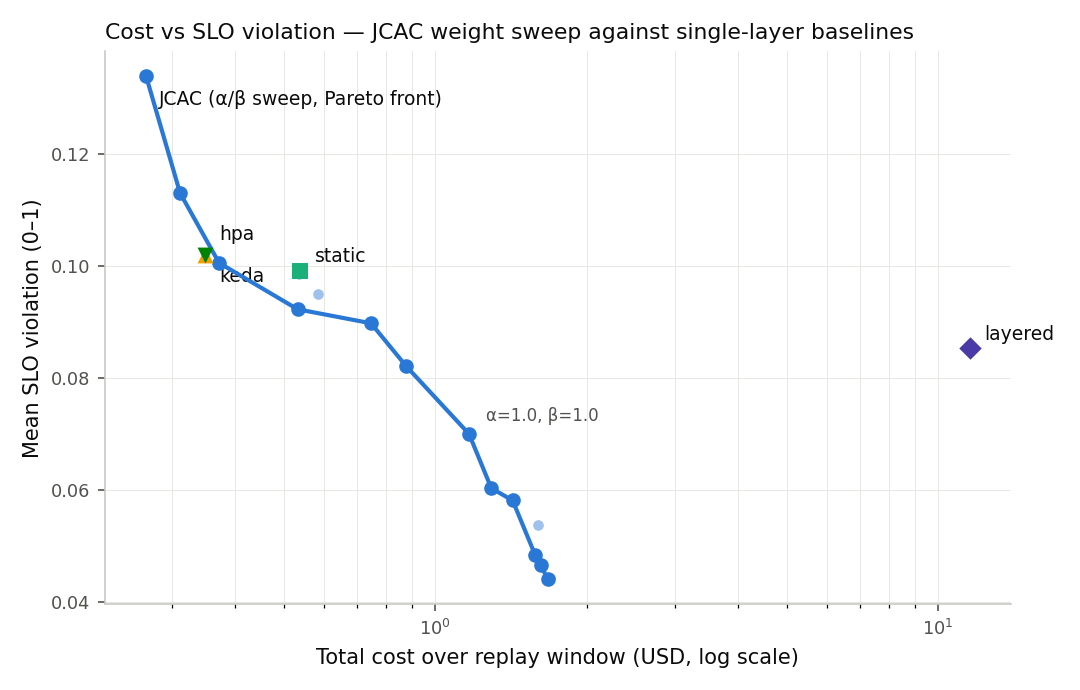
\includegraphics[width=\linewidth]{figures/jcac-pareto}
  \caption{Cost vs.\ mean SLO violation on the Azure trace replay. Small
  dots: JCAC $(\alpha,\beta)$ sweep at $\gamma{=}0.5$; line: its Pareto
  front. Single-layer baselines cannot reach below the front: the
  \textsf{layered} stack of three locally tuned controllers costs
  ${\sim}7\times$ more than JCAC's default point with worse violation.}
  \label{fig:jcac-pareto}
\end{figure}

Absolute dollar and latency values are artifacts of the simulator's
calibration and carry no external validity; the claims this section makes
are ordinal --- domination and ranking under identical assumptions.
Live-cluster measurements are the subject of \S\ref{sec:evaluation}.
